\section{Design}
We created the chatbot for CGNet Swara, a citizen journalism platform where users give a missed call to a number, whereupon they are called back and can press `1' to report a story and `2' to hear the verified, fact-checked stories others have reported (this is cheaper than an inbound toll-free number). In the organizations 10 year history, over 100,000 unique users have called this number to report or listen, while more than 20,000 stories have been published from 6300 unique users. An internal survey found that roughly 30\% of their users had associated WhatsApp accounts, prompting our team to explore how users could submit and listen to stories through WhatsApp.

The full interaction flow of the chatbot is shown in Figure~\ref{fig:flow}. The choice for language was Hindi written in English characters. If the user sends a message other than from the WhatsApp attachments (audio, video, image, contact card and location), the bot replies with a randomly chosen story among the set of latest stories and a welcome message that includes the link to our chatbot, which can be forwarded to other users, as shown in Figure~\ref{fig:menu_contactcard_anony}. 

\begin{figure*}[htb!] 
    \centering
    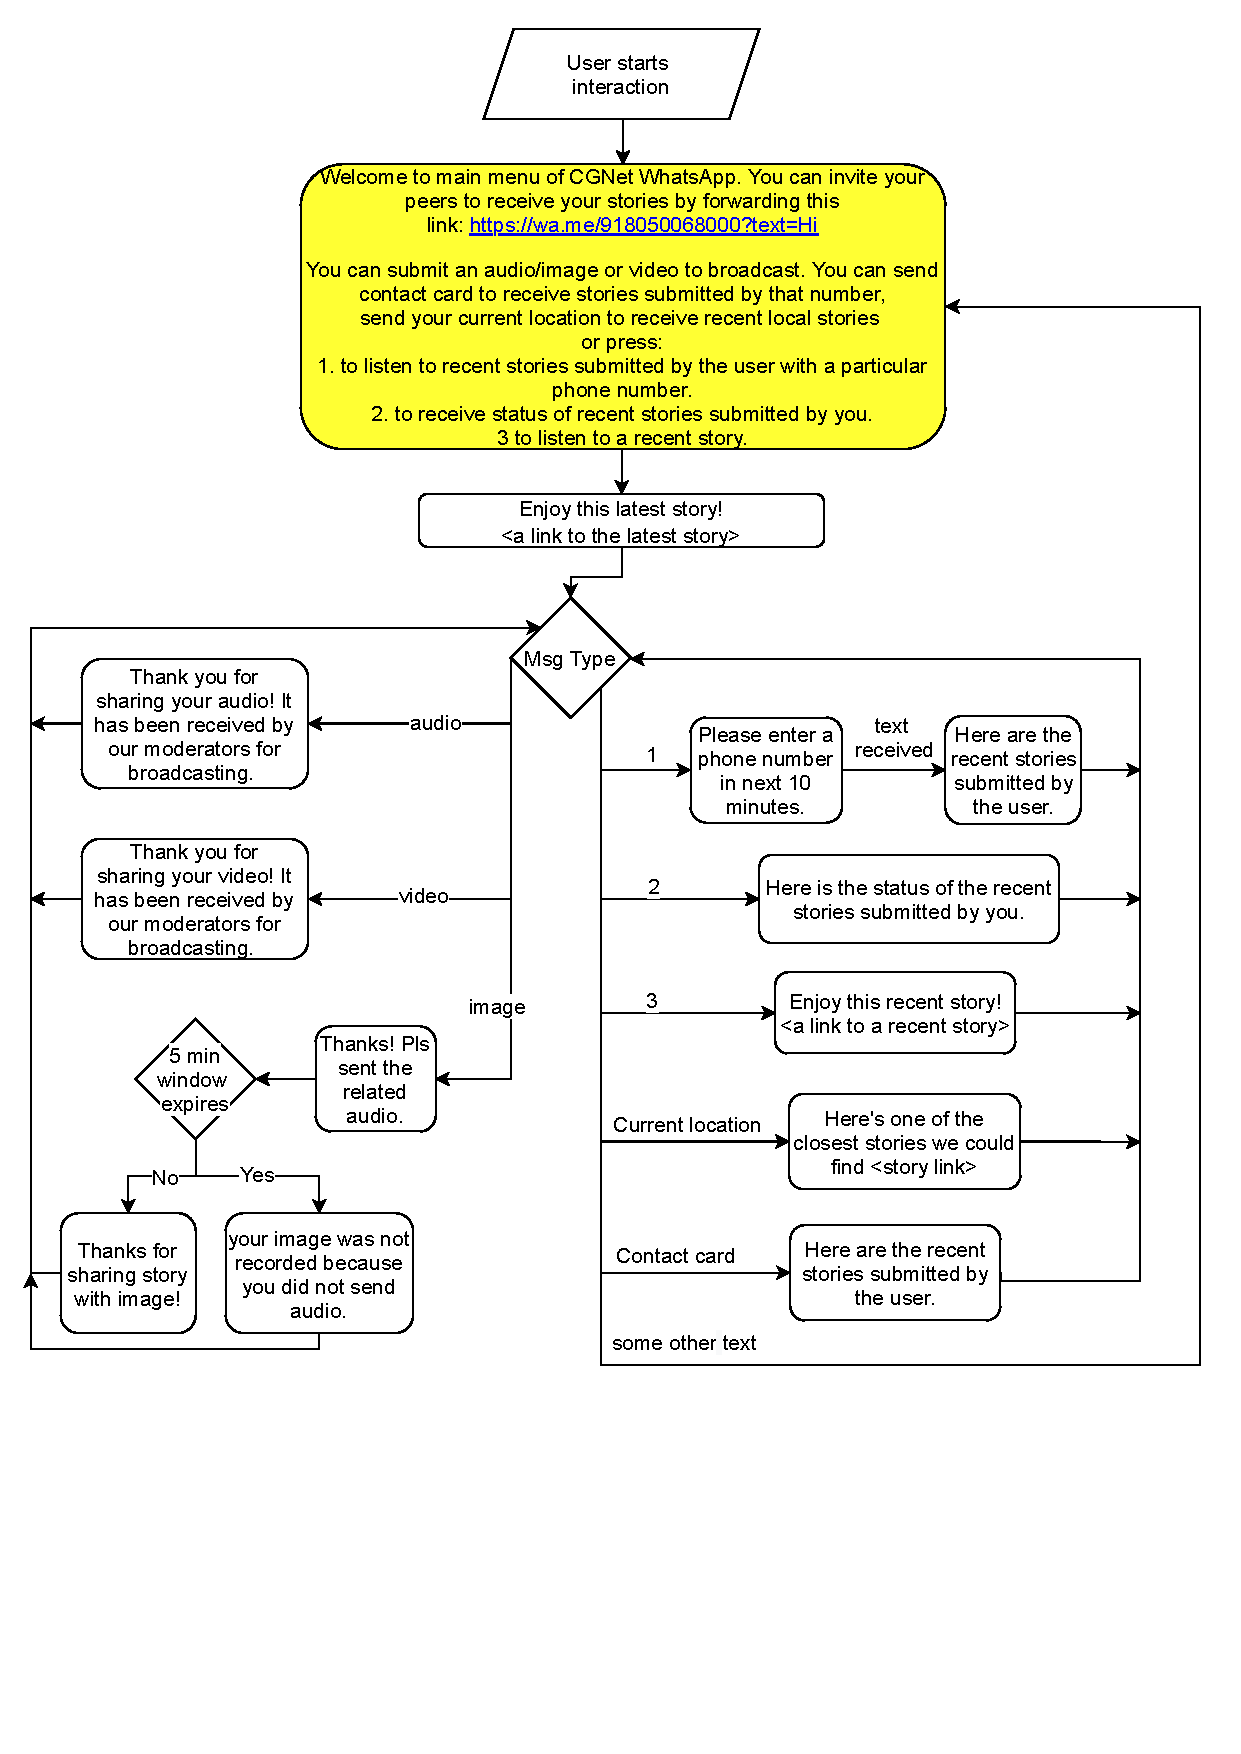
\includegraphics[width = \textwidth]{images/Final_PDF_Flow7.pdf}
    \caption{Interaction flow for content acceptance and dissemination.}
    \label{fig:flow}
    \Description[A  float image]{The image shows the interaction flow for content acceptance and dissemination through the deployed WhatsApp chat bot. The diagram begins when a user starts interaction by sending a message to the chat bot. The flow chart proceeds to display the main menu message and a link to the latest story. Then the left part of the flow chart shows that users can send audio, video or image attachments in WhatsApp to submit their stories. If a user submits image then he is asked to submit a corresponding audio story. On the right side of the flow chart, various ways of how users can request stories or status of their stories is shown. }
\end{figure*}

One of our main design constrains arose from the fact that we were designing for users who may be too low literate to navigate text content. Medhi argues that textual non-literacy is correlated with reduced cognitive skills required to navigate information architectures~\cite{medhi_2015_user}, convincing us to sacrifice greater functionality for simplicity. If a user sends a WhatsApp attachment such as an audio or video file, it is assumed to be a story submission and there is no confirmation required as users may not know how to read or type. In case more technologically proficient users want a photo to go along with their story, they can send an image, which is then followed by a request for the corresponding audio story, as shown in Figure~\ref{fig:video_image}. We tried to guide users at each step of their interaction journey through an instruction or acknowledgment based reply, although this can be tricky as users may be unable to understand these messages.

\begin{figure}[t]
    \centering
    \begin{subfigure}[b]{0.48\textwidth}
        \centering
        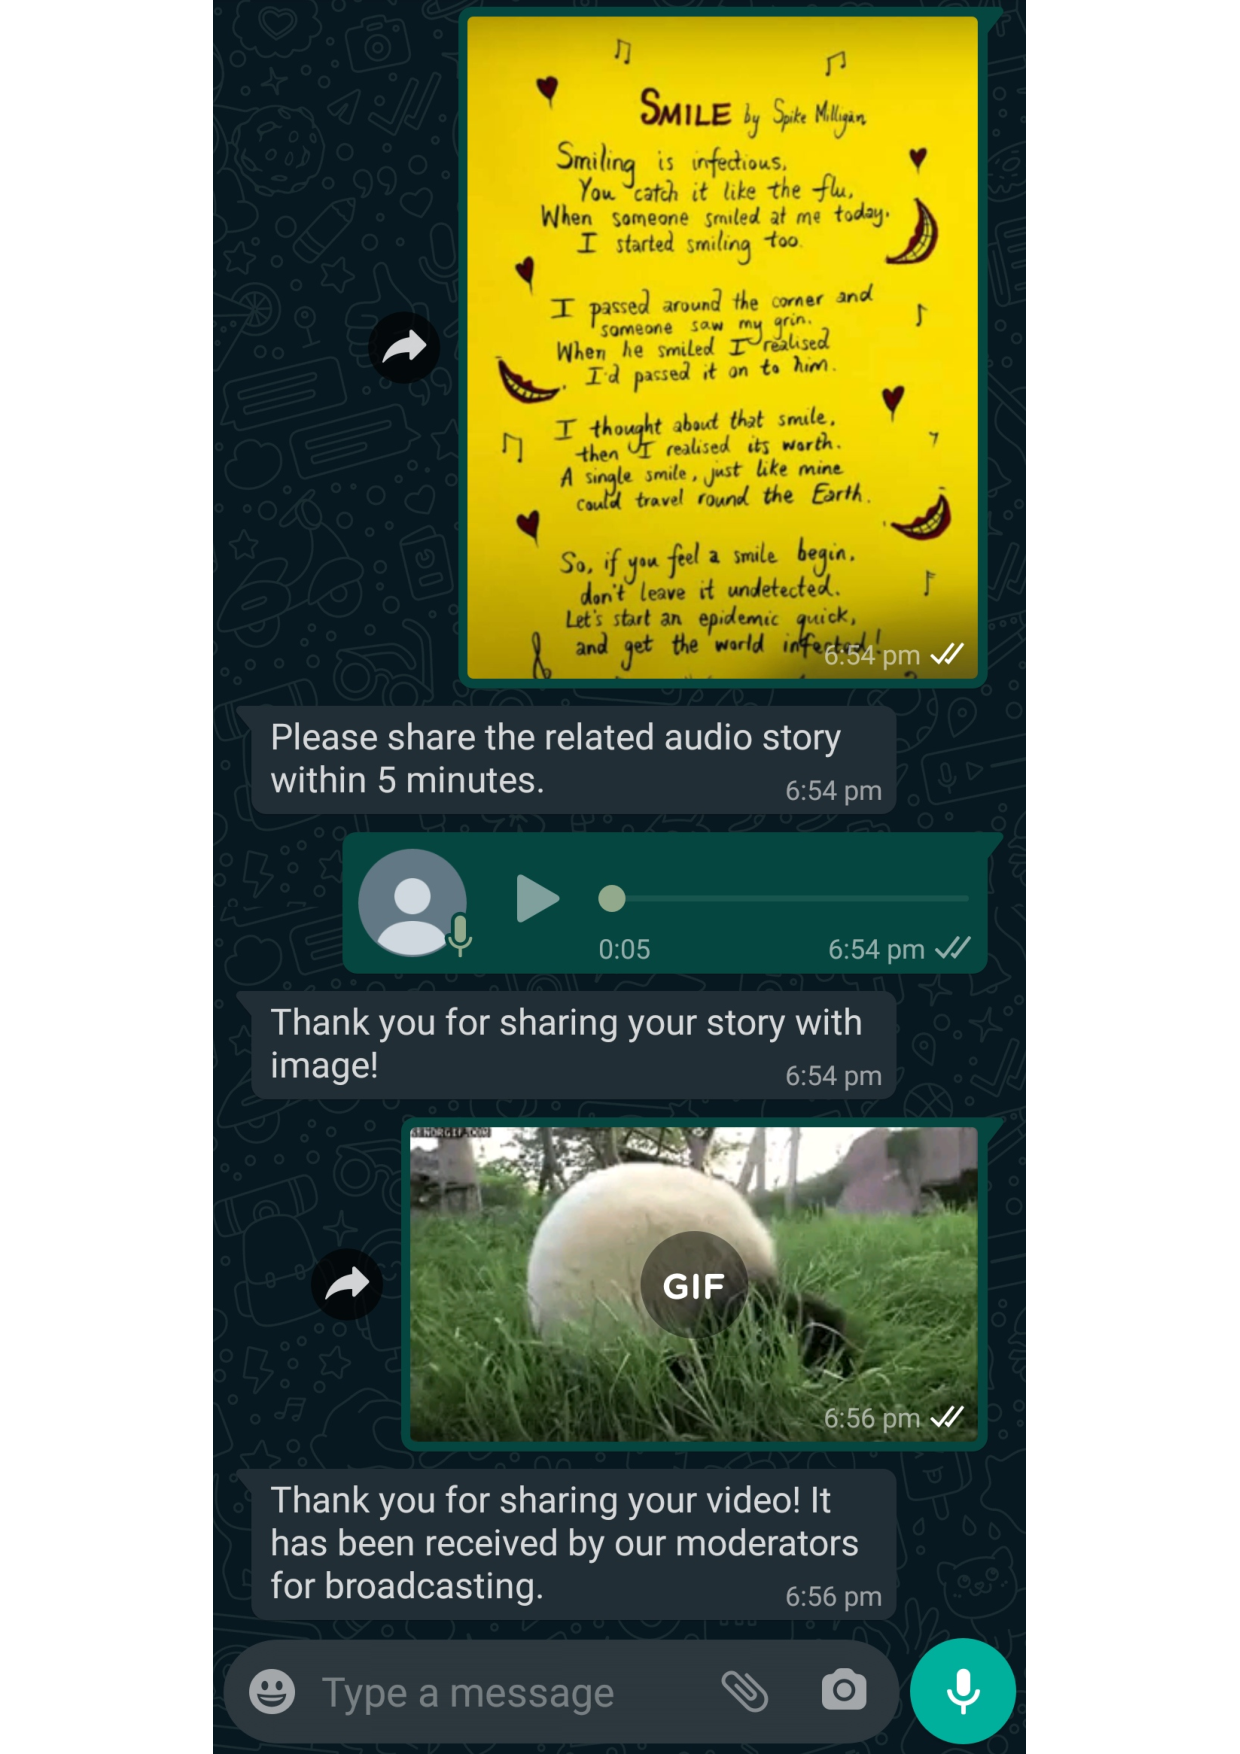
\includegraphics[height=\textwidth]{images/receive_image_video_PDF.pdf}
    \caption{Receiving video and image-based audio stories from user.}
    \label{fig:video_image}
    \end{subfigure}
    \hfill
    \begin{subfigure}[b]{0.48\textwidth}
         \centering
         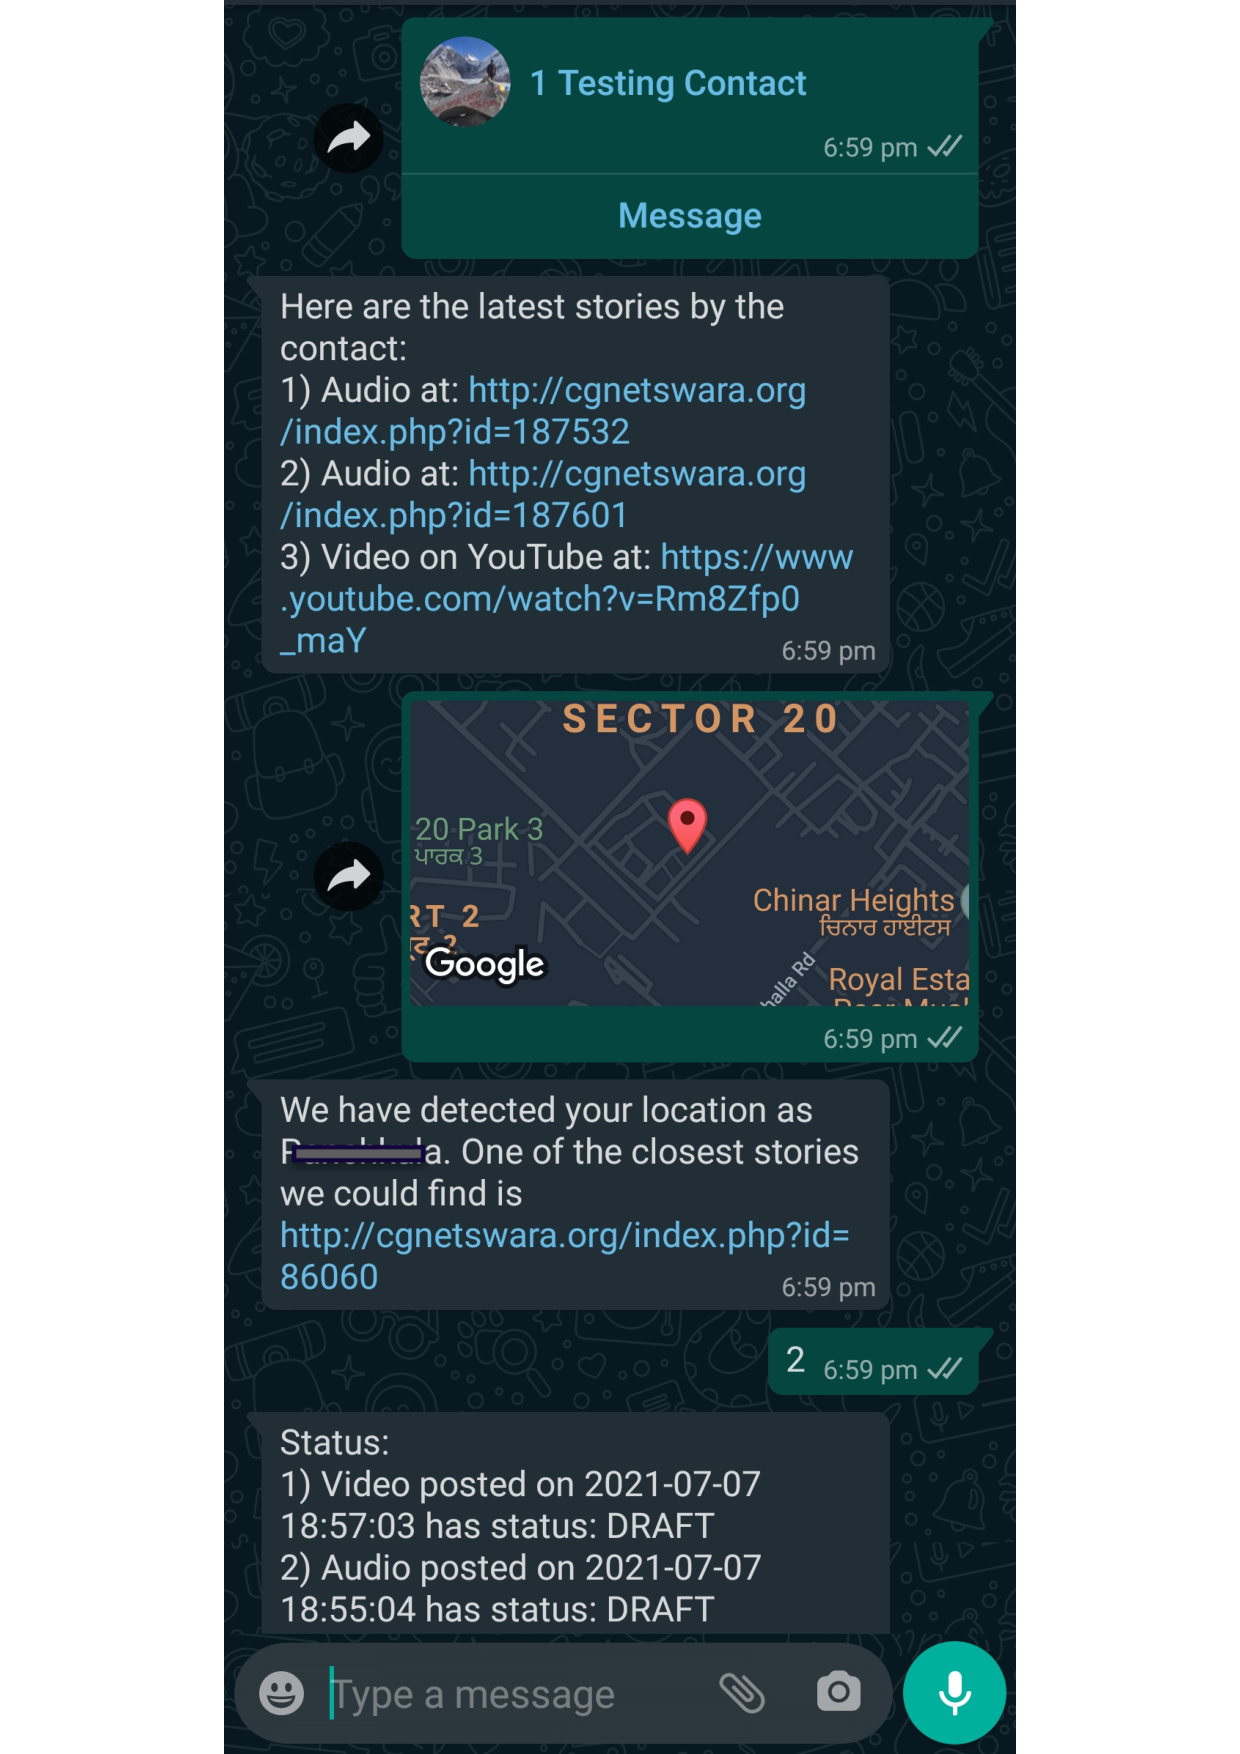
\includegraphics[height=\textwidth]{images/send_location_ccard_PDF.pdf}
    \caption{Sending latest stories and status to user.}
    \label{fig:menu_contactcard_anony}
    \end{subfigure}
    % \hfill
    % \begin{subfigure}[b]{0.31\textwidth}
    %      \centering
    %      \includegraphics[height=1.5\textwidth]{images/location.png}
    % \caption{Sending a location based story to user. Display of the features to send status of stories and the latest story.}
    % \label{fig:location}
    % \end{subfigure}
    \caption{Demo of the deployed chatbot.}
    \label{fig:two graphs}
    \Description[Two float images]{First image shows that user can send an image, followed by audio and a video to chatbot to submit his stories. The second image shows that user can send a contact card to received latest stories submitted from that phone number. It also shows that user can submit current location to receive latest local stories from that area and when user presses 2, he received the status of recent stories submitted by him.}
\end{figure}

We also designed our chat interface so that it could be operated with minimal number of steps and without any textual input. If users want to listen to more stories, they can do that by typing in `3' at anytime, without having to return to the main menu. Users may also request for stories reported by another user by typing in `1' and then entering the phone number of the person whose stories they wish to listen to, or by directly sending a contact card attachment (Figure~\ref{fig:menu_contactcard_anony}). Similarly, users can listen to stories reported by users in their district by simply sending the location attachment (through the 'Send current location' feature). Additionally, more literate users can request for the status of their unpublished stories by typing in `2'- a personalised feedback mechanism that could not only help increase their engagement but also build accountability in the organisation so that users can complain to the staff if their story has been left unattended. 

%While the IVR platform of the organisation has shown remarkable promise in reaching populations too poor to own a smartphone, too low literate to navigate text content or too remote to access the internet, they have also had difficulty in scaling up due to inefficient cost structures compared to internet platforms. A smartphone app has been deployed to provide more functionality to users than IVR like sharing audios, saving media on phone storage, however, there are additional overheads of installation and training. On the contrary, WhatsApp is one of the most used social media platforms in rural India~\cite{statista_2018_social, tandon_2016_rural}. The WhatsApp channel has been thus designed as a supplement to and not a substitute of IVR or smartphone app. 

A second set of design constraints came from our team having to integrate as far as possible with the existing workflow used by CGNet. For example, editing and reviewing stories submitted via IVR takes place on the open-source loudblog moderation platform, forcing us to modify its capabilities to accept video submissions made over WhatsApp. A regular account on WhatsApp would not have allowed us to take audio or video submissions directly onto the moderation platform, prompting us to explore the API which comes with a fixed cost of USD 500 per month and has its own set of design constraints. WhatsApp bots can reply for free within a 24 hour window from the user's last message, while initiating a conversation outside this window incurs marginal costs of USD 0.005 per message and also requires both permission from the user and that the message be pre-approved by Facebook. To minimize cost and complexity, we designed the bot such that it only replies to users.
% 
% or those from another user by sharing their contact card.

% \begin{figure}
%     \centering
%     \includegraphics[height= 0.7\textwidth]{images/video_image_dark.png}
%     \caption{Receiving video and image based audio stories from user.}
%     \label{fig:video_image_dark}
% \end{figure}

% \begin{figure}
%     \centering
%     \includegraphics[height= 0.8\textwidth]{images/video_image.jpg}
%     \caption{Receiving video and image based audio stories from user.}
%     \label{fig:video_image}
% \end{figure} 

%Similarly, instead of asking users to optionally submit an image associated with an audio story, the bot asks for a compulsory corresponding audio when a user submits an image. The former method would add one more level of depth as it would require users to input an additional message to confirm if an audio submitted after an image is associated with it, therefore was rejected to reduce cognitive load of users. . For the same reason, users are not asked to press a button to confirm their submission, unlike in the case of IVRs.    

The third and final set of factors influencing our design was the needs and capacities of CGNet Swara. To save space and reduce load on their IVR server, videos are hosted on YouTube and dissemination of stories on WhatsApp is done through sending links instead of the actual media file. Audio is automatically extracted from videos received via WhatsApp, so that they can be separately edited and played over the IVR channel. We also found that many of the staff reporters earlier faced issues with space on their phone for storing video or audio interviews they took while in the field, which was mitigated by having them simply send those media files to the WhatsApp chatbot we designed.

In the future, we have plans to introduce a special ``moderator mode'' on the WhatsApp bot that would reduce the workload of editors on the moderation platform. Experienced reporters in the field would be able to type in metadata about the story they are reporting, such as its title and description, which are currently filled in by moderators.

%Users not owning a smartphone, can have their story reported by reporters on field visits, who can access a special 'Moderator' mode. This feature specifically helps to distinguish between the reporter and owner of the story, i.e, through this feature the owner of story can be identified even if his/her story has been submitted by a reported. Additionally, reporters can type in metadata, such as its title and description to reduce the work of the backend moderation team. This metadata could then be manually typed in the loudblog website. 


%To save space on and distribute load from the server, YouTube is chosen over the organisation's front facing website for hosting final videos, and to leverage other advantages like global outreach, richer viewer analytics and monetizability. Due to internet constraints of users in rural areas, the dissemination of stories was done by sending links to media hosted on YouTube or on the organisation website, instead of actual media file.



% \begin{figure}
%     \centering
%     \includegraphics[width= 0.8\textwidth]{images/phone_stories.png}
%     \caption{Sending users stories submitted by the contact number typed by them.}
%     \label{fig:send_phone_story}
% \end{figure}

% \begin{figure}
%     \centering
%     \includegraphics[width=0.8 \textwidth]{images/status_stories.png}
%     \caption{Sending users the status of the latest stories submitted by them. Like other features, users can access this feature after the main menu or at any other stage of the interaction flow.}
%     \label{fig:send_status}
% \end{figure}

% 
\section{Deployment}

In 28 days of deployment, a total of 236 stories were reported by 25 unique users, of which 126 have been fact-checked, verified and published online (Table~\ref{tab:usage_data}). Only 2 video stories have been published out of 37 submissions, due in part to the CGNet moderators lacking video editing skills. One of the videos was sent by an old man who sang a song,

\textit{``You would see that we will defeat Corona. We will not participate in mass gathering. You would see that we will defeat Corona. We will not hug or shake hands with each other...''
}
%As seen in Table~\ref{tab:usage_data}, 

The majority of stories comprise accounts of violence inflicted by insurgent or government forces (CGNet operates in a region experiencing more than 30 years of civil war). This may be due to CGNet preferring to first test the chatbot with their own reporters, who are tasked with reporting stories of victims caught in the conflict, before publicizing it to other citizen journalists who currently use their IVR channel as a cultural repository and to report longstanding community issues. The chatbot nevertheless received 45 stories centered around basic governance problems that show how citizen journalists can speak truth to power. For example, despite government claims of electrifying all villages in India, we received the following report from a user in the Central Southern state of Telangana;

\textit{``Since past 15 years, the villagers are facing electricity problems due to which we do not have proper lighting facility here. We have to stay in dark during night times due to lack of electricity. Advanced facilities are also not available. I appeal to you all for help.''
}

Only 2 impact stories were recorded where users updated us that the problem they reported earlier had been resolved. Future work will need to look more carefully at developing mechanisms to solve issues raised on the platform.

%Our WhatsApp based citizen journalism platform has been live for 28 days at the time of writing. The usage numbers  after 28 days of deployment are shown in . The organisation has not publicized the presence of their WhatsApp channel, preferring to first test it with their own staff reporters.

\begin{table}[!htbp]
    \centering
    \caption{Usage data for 9 weeks of deployment.}
    \begin{tabular}{l l}
        \noalign{\smallskip}\midrule
        Parameter & Count \\
        \noalign{\smallskip}\midrule
        Total stories received via WhatsApp &	539  \\
        Stories published on web & 218	 \\
        Distinct users	& 27 \\
        Total video stories received & 93	\\
        Video stories published & 4	\\
        \noalign{\smallskip}\hline
    \end{tabular}
    
    \label{tab:usage_data}
\end{table} 


% \begin{table}[!htbp]
%     \centering
%     \caption{Classification of Stories}
%     \label{tab:classification}
%     \begin{tabular}{c c}
%         \noalign{\smallskip}\hline
%         Story Type & Count  \\
%         \hline\noalign{\smallskip}
%         Victim &	78 (62\%) \\
%         Problems & 45 (36\%)	 \\
%         Impact	& 2 (2\%)\\
%         Song & 1 (<1\%)	\\
%         \noalign{\smallskip}\hline
%     \end{tabular}
% \end{table} 


%\begin{table}[h]
%\caption{Analysis of stories submitted via WhatsApp which have been published online.}
%    \begin{subtable}[h]{0.49\textwidth}
%    \centering
%    \caption {Classification of stories.}
%    \begin{tabular}{l l}
%        \noalign{\smallskip}\midrule
%        Story Type & Count   \\
%        \noalign{\smallskip}\midrule
%        Victim &	117 (53.67\%) \\
%        Problems & 81 (37.16\%)	 \\
%        Song & 8 (3.67\%)	\\
%        Impact	& 6 (2.76\%)\\
%        For Awareness & 4 (1.84\%) \\
%        Story & 2 (<1\%)	\\
%        \noalign{\smallskip}\bottomrule
%    \end{tabular}
%    \label{tab:classification_stories}
%    \end{subtable}
%    \hfill
%    \begin{subtable}[h]{0.49\textwidth}
%    \centering
%     \caption {Classification of problem stories.}
%    \begin{tabular}{l l }
%         \noalign{\smallskip}\midrule
%         Problem Type  & Count \\
%        \noalign{\smallskip}\midrule
%        Water  & 35 (43.21\%)  \\
%        Ration card  & 8 (9.88\%)	\\
%        Road & 13 (16.05\%)  \\
%        Electricity & 4 (4.94\%) \\
%        Pension & 11 (13.58\%) \\
%        Miscellaneous & 10 (12.34\%) \\
%        \noalign{\smallskip}\bottomrule
%    \end{tabular}
%   
%    \label{tab:classification_problem}
%    \end{subtable}
%    \label{fig:smartphone_features}
%    
%\end{table}

\begin{table}[h]
\caption{Analysis of stories submitted via WhatsApp which have been published online.}
\centering

\begin{tabular}{@{}c@{}}
    %\begin{subtable}[h]{0.49\textwidth}
\multicolumn{1}{@{}c@{}}{\bf (a) Classification of stories.}\\ \hline
    
    %\caption {Classification of stories.}
\tabcolsep12pt
    \begin{tabular}{l l}\hline
        
        Story Type & Count   \\ \hline
        
        Victim &	117 (53.67\%) \\
        Problems & 81 (37.16\%)	 \\
        Song & 8 (3.67\%)	\\
        Impact	& 6 (2.76\%)\\
        For Awareness & 4 (1.84\%) \\
        Story & 2 (<1\%)	\\
        \hline
    \end{tabular} \\\\
    %\label{tab:classification_stories}
    %\end{subtable}
\multicolumn{1}{@{}c@{}}{\bf (b) Classification of problem stories.}\\ \hline
    %\begin{subtable}[h]{0.49\textwidth}
    %\centering
     %\caption {Classification of problem stories.}
\tabcolsep13pt
    \begin{tabular}{l l }
         \hline
         Problem Type  & Count \\
        \hline
        Water  & 35 (43.21\%)  \\
        Ration card  & 8 (9.88\%)	\\
        Road & 13 (16.05\%)  \\
        Electricity & 4 (4.94\%) \\
        Pension & 11 (13.58\%) \\
        Miscellaneous & 10 (12.34\%) \\
        \hline
    \end{tabular}
   \end{tabular}

    %\label{tab:classification_problem}
    %\end{subtable}
    \label{fig:smartphone_features}
    
\end{table}